We can imagine the components of the mind as white boxes which inform other components by their very functioning --- however, this does not lend itself to easy implementation. Instead, we can emulate this behaviour via a \caps{message space}, from which individual components take their input and into which they put their output. A \caps{component} is then a local processing unit which continuously scans the message space, running messages through its \caps{filter}. If the filter detects a relevant message, it is then passed to the \caps{interpreter}, which parses the message into the needed format and hands it over to the \caps{processor}. The processor, after having finished, puts its output back into the message space for other components to read. Figure~\ref{fig:global} illustrates this scheme. Note the lack of explicit hierarchical structure and central organising units.

\begin{figure}
	\begin{center}
		\begin{tabular}{l l}
			\toprule
			Symbol & Description\\
			\midrule
			
			\begin{minipage}[t]{0.2\textwidth}
				
\includegraphics[width=80pt]{figs/legend_proc.png}
			\end{minipage}
			 & Processing component\\
			
\includegraphics[width=80pt]{figs/legend_choice.png} & Choice\\
			
\includegraphics[width=50pt]{figs/legend_container.png} & Data container (Queue, List, etc.)\\
			
\includegraphics[width=50pt]{figs/legend_data.png} & Data\\
			
\includegraphics[width=30pt]{figs/legend_generator.png} & Stream generator\\
			
\includegraphics[width=50pt]{figs/legend_imaginary.png} & Counterfactual (imaginary) data\\
			\bottomrule
		\end{tabular}
	\end{center}
	\caption{Notation for the diagrams in this and the following sections.}
	\label{fig:diagramNotation}
\end{figure}
%
\begin{figure}[!h]
	\centering
	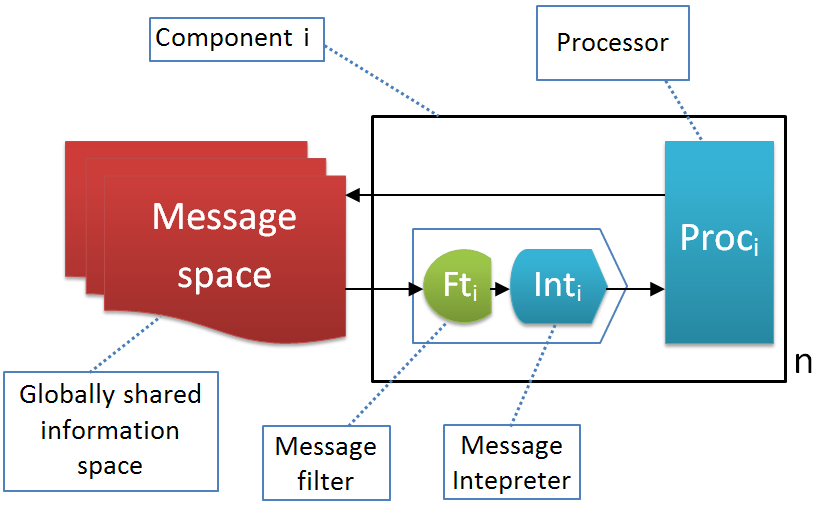
\includegraphics[width=400pt]{figs/global.png}
	\caption{Global neural architecture.}
	\label{fig:global}
\end{figure}

However, as I'll show in the next section, this model is generic enough to accommodate such special-purpose structures. Figure~\ref{fig:global} shows the message-passing scheme, but it also specifies a graph in which the nodes are the components and fixed, while the edges are the accepted messages and are determined by the nodes; through their filters, components control the shape of the graph. By imposing invariants on these filters, we can have the graph take any shape we desire. In particular, we can model the kinds of structures that occur in many other cognitive models and in empirical research: central organisers, sequences of components (``pipelines''), localized messages affecting only a small part of the mind, a component reading its own messages, loops and iterative messages between two or more components et cetera.

\pagebreak

\paragraph{Messages}

We may now ask how such messages between components are structured. Here, I make two empirical claims:
\begin{enumerate}
	\item messages have a priority and
	\item they are effectively unstructured.
\end{enumerate}

\begin{figure}[!h]
	\centering
	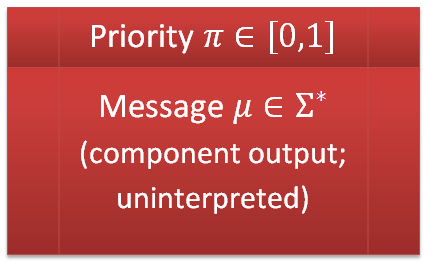
\includegraphics[width=150pt]{figs/message.png}
	\caption{Structure of a neural message.}
	\label{fig:message}
\end{figure}

To the best of my knowledge, the veracity of either has thus far not been determined by neuroscience. For the first, Marvin Minsky's ``The Emotion Machine'' provides some circumstantial evidence \cite[p. 222]{emotionMachine}:

\begin{quote}
	Of course, when one activates two or more Critics or Selectors, this is likely to cause some conflicts, because two different resources might try to turn on a third resource both {\em on} and {\em off}. To deal with this, we could design the system to use various policies like these:
	
	\begin{enumerate}
		\item Choose the resource with the highest priority.
		\item Choose the one that is most strongly aroused.
		\item Choose the one that gives the most specific advice.
		\item Have them all compete in some ``marketplace''.
	\end{enumerate}
\end{quote}

The selection strategies Minsky lists imply that there is some mechanism in the brain to determine the urgency of a signal. While it is possible that higher brain functions like reasoning or affect make an additional, rational evaluation, sensations like intense pain, bright lights, or great sadness can likely be communicated most easily by the appropriate components causing a flood of activity which, by its very intensity, informs other components of the urgency of their messages.

The second claim --- that messages are essentially unstructured --- means that there is no common, agreed-upon format in which they are stored. In addition to the evolutionary implausibility of such a format being created, an unstructured message format is in line with the white-box nature of components: since components merely ``listen in'' on others, and since each components will have its own pattern of activity, a listener would simply have to try and make sense of this activity as best it could. The proposed structure of messages is thus shown in Figure~\ref{fig:message}: every message comprises a priority header, together with an unstructured body which, for our purposes, is simply a string of bits.

\paragraph{Filters} Before a component can respond to a message by another, such a message must be assessed for the presence of relevant information. Conceptually, this happens via a \caps{filter} in each component, which pattern-matches incoming messages and, if a certain threshold is reached, signals relevance and hands the message over the \caps{interpreter} for parsing. Figure~\ref{fig:filter} shows such a filter: it is composed of a directed graph of nodes, and a node is activated if it detects some specific content in the message. Nodes, in turn, are connected via edges of strength $\in [0,1]$. When a node is activated, it sends a charge proportional to the strength of its link to its neighbours, contributing to their activation as well. Some nodes are marked as {\em output nodes}; if enough such output nodes become activated, the message is deemed to be sufficiently relevant. This model of filters is inspired by the {\em spiking neural P Systems} of Georghe Pa\u{u}n et al. (\cite[p. 337]{membraneComputing} and \cite{spikingNeural}), in which charges sent along directed graphs of neurons are used to compute functions.

\begin{figure}[!h]
	\centering
	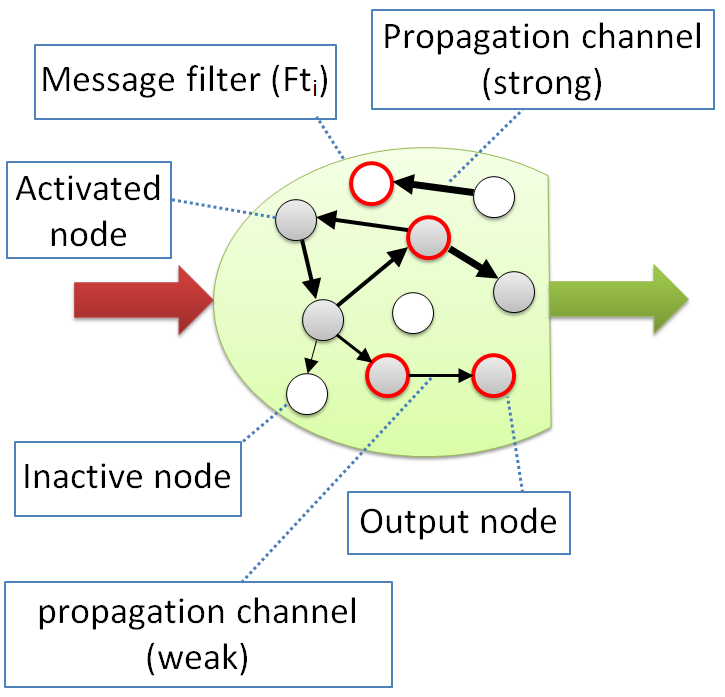
\includegraphics[width=168pt]{figs/filter.png}
	\caption{A pattern-matching filter for a component $C_i$.}
	\label{fig:filter}
\end{figure}